\documentclass[tikz]{standalone}
\usepackage{color}
\usetikzlibrary{bayesnet}

\begin{document}

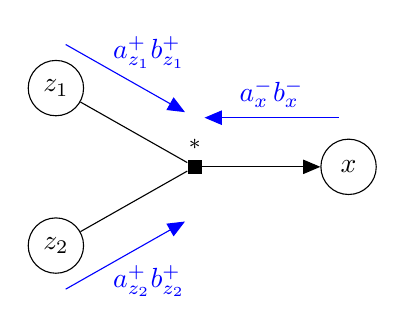
\begin{tikzpicture}
      \centering
      \node[latent] (x)  {$x$} ;
      \node[latent, left=3 of x, yshift=+1cm] (z1) {$z_1$} ;
      \node[latent, left=3 of x, yshift=-1cm] (z2) {$z_2$} ;

      \factor[left=1.5 of x] {D} {$*$} {z1,z2} {x} ;

      \node[above=0.5 of z1.center] (s1) {} ;
      \node[above=0.5 of D.center] (t1) {};
      \draw[->, blue] (s1) -- (t1) node[midway,above,xshift=+2ex] {$a_{z_1}^+ b_{z_1}^+$} ;

      \node[below=0.5 of z2.center] (s2) {} ;
      \node[below=0.5 of D.center] (t2) {};
      \draw[->, blue] (s2) -- (t2) node[midway,below,xshift=+2ex] {$a_{z_2}^+ b_{z_2}^+$} ;

      \node[above=0.5 of x.center] (s3) {} ;
      \node[above=0.5 of D.center] (t3) {};
      \draw[->, blue] (s3) -- (t3) node[midway,above] {$a_x^- b_x^-$} ;
\end{tikzpicture}

\end{document}
